\documentclass[11pt]{article}
\usepackage{diagbox}
\usepackage{stmaryrd}
\usepackage{mathtools}
\usepackage{graphicx}
\usepackage{hyperref}
\usepackage[utf8]{inputenc}
\usepackage{amsmath,amsthm,amsfonts,amssymb,amscd}
\usepackage{tikz}
\usepackage{xeCJK}
\usepackage{physics}
\usepackage{multirow,booktabs}
% \usepackage[table]{xcolor}
\usepackage{fullpage}
\usepackage{lastpage}
\usepackage{unicode-math}
\usepackage{enumitem}
\usepackage{fancyhdr}
\usepackage{mathrsfs}
\usepackage{wrapfig}
\usepackage{setspace}
\usepackage{calc}
\usepackage{multicol}
\usepackage{cancel}
\usepackage[retainorgcmds]{IEEEtrantools}
\usepackage[margin=3cm]{geometry}
\usepackage{amsmath}
\DeclareMathAlphabet{\mathcal}{OMS}{cmsy}{m}{n}
\let\mathbb\relax
\DeclareMathAlphabet{\mathbb}{U}{msb}{m}{n}
\newlength{\tabcont}
\setlength{\parindent}{0.0in}
\setlength{\parskip}{0.05in}
\usepackage{empheq}
\usepackage{framed}
\usepackage[most]{tcolorbox}
\usepackage{xcolor}
\linespread{1.2}
\graphicspath{{./}}
\setCJKmainfont[AutoFakeBold = 3, AutoFakeSlant = 4]{BiauKaiTC}
\colorlet{shadecolor}{orange!15}
\parindent 0in
\parskip 12pt
\geometry{margin=1in, headsep=0.25in}
\graphicspath{{./}}
\theoremstyle{definition}
\newtheorem{thr}{Theorem}
\newtheorem{lma}{Lemma}
\newtheorem{defn}{Definition}
\newtheorem{reg}{Rule}
\newtheorem{exer}{Exercise}
\newtheorem{note}{Note}
\newtheorem{asmp}{Assumption}
\begin{document}
\setcounter{section}{0}
\title{Title}

\thispagestyle{empty}
\begin{center}
  {\large \bf HTML HW6} \\ 
  B12901022 廖冠豪
\end{center}
\section*{5}
Consider the case where $\vb{z}_n^T = [1, \vb{x}_n^T]$ is fed indo $D_1$
\begin{align*}
  \min_{\vb{\alpha}}\quad&\frac{1}{2}\sum^N_{n = 1}\sum^N_{m = 1}\alpha_n\alpha_my_ny_m\vb{z}_n^T\vb{z}_m - \sum_{n = 1}^N\alpha_n \\ 
  \text{Subject to}\quad &\sum^N_{n = 1}y_n\alpha_n = 0, \quad 0 \leq \alpha_n \leq C\quad\forall n \in \{1, 2,\dots,N\}
\end{align*}
Notice that
\[
  \vb{z}_n^T\vb{z}_m = \begin{bmatrix}1 &\vb{x}_n^T\end{bmatrix}\begin{bmatrix}1 \\ \vb{x}_m\end{bmatrix} = 1 + \vb{x}_n^T\vb{x}_m
\]
So $D_1$ becomes
\begin{align*}
  \min_{\vb{\alpha}}\quad&\frac{1}{2}\sum^N_{n = 1}\sum^N_{m = 1}\alpha_n\alpha_my_ny_m\vb{x}_n^T\vb{x}_m + \frac{1}{2}\sum^N_{n = 1}\sum^N_{m = 1}\alpha_n\alpha_my_ny_m - \sum_{n = 1}^N\alpha_n \\ 
  \text{Subject to}\quad &\sum^N_{n = 1}y_n\alpha_n = 0, \quad 0 \leq \alpha_n \leq C\quad\forall n \in \{1, 2,\dots,N\} \\
\end{align*}
The only difference between this and the original form of the problem is the $\frac{1}{2}\sum^N_{n = 1}\sum^N_{m = 1}\alpha_n\alpha_my_ny_m$ term
\[
  \frac{1}{2}\sum^N_{n = 1}\sum^N_{m = 1}\alpha_n\alpha_my_ny_m = \sum^N_{m = 1}\left(\alpha_my_m\sum^N_{n = 1}\alpha_ny_n\right)
\]
Since we have the constraint $\sum^N_{n = 1}y_n\alpha_n = 0$, we know that the term above is $0$, and the two optimization problem in fact solve for the same $\alpha$ \\ 
Let the solution to the original problem be $(b, \vb{w}, \alpha)$

Hence, $\alpha^\star = \alpha$ \\
From the lecture slides, we know that $\vb{w} = \sum^N_{n = 1}\alpha_ny_n\vb{z}_n$, so we have
\[
  \vb{w} = \sum^N_{n = 1}\alpha_ny_n\vb{x}_n,\quad\tilde{\vb{w}^\star} = \sum^N_{n = 1}\alpha_ny_n[1\ ,\vb{x}_n^T]^T
\]
So 
\begin{align*}
  \tilde{\vb{w}^\star} &= [\sum^N_{n = 1}\alpha_ny_n\ ,\vb{w}]^T \\ 
  &= [0\ \vb{w}]^T\quad(\text{Because we have the constraint }\sum^N_{n = 1}\alpha_ny_n = 0)
\end{align*}
Hence $\vb{w}^\star = \vb{w}$ \\
Also from the lecture slides, $b = y_s - \vb{w}^T\vb{z}_s$, where $\vb{z}_s$ is some free support vector. \\ 
So, with some $0 < \alpha_s < C$ 
\begin{align*}
  b^\star &= y_s - \tilde{\vb{w}^\star}^T\vb{z}_s \\ 
  &= y_s - [0\ \vb{w}][1\ \vb{x}_s]^T \\ 
  &= y_s - \vb{w}^T\vb{x}_s
\end{align*}
And 
\begin{align*}
  b &= y_s - \vb{w}^T\vb{x}_s
\end{align*}
Hence we also see that $b^\star = b$
\par 
From the analysis above, we see that $(b^\star, \vb{w}^\star ,\alpha^\star) = (b, \vb{w}, \alpha)$, and hence $(b^\star, \vb{w}^\star ,\alpha^\star) = (b, \vb{w}, \alpha)$ is an optimal solution to the original problem.
\newpage
\section*{6}
Original problem:
\begin{align*}
  (P)\quad &\min_{\vb{w}, b, \xi} \quad \frac{1}{2}\vb{w}^T\vb{w} + C\sum^N_{n = 1}\xi_n \\ 
  \text{Subject to}\quad& y_n(\vb{w}^T\Phi(\vb{x}_n) + b)\geq 1 - \xi_n, \text{for }n = 1, 2,\dots,N \\ 
  &\xi_n \geq 0, \text{for }n = 1, 2, \dots, N \\ 
  & y_0(\vb{w}^T\Phi(\vb{w}_0) + b) \geq 1
\end{align*}
Define $\vb{z}_n = \Phi(\vb{w}_n)$ \\
This is equivalent to 
\begin{align*}
  \min_{b, \vb{w}, \xi}\left(\max_{0\leq \alpha_n, 0\leq \beta_n}\frac{1}{2}\vb{w}^T\vb{w} + C\sum^N_{n = 1}\xi_n + \sum^N_{n = 1}\alpha_n(1 - \xi_n - y_n(\vb{w}_n^T\vb{z}_n) + b) + \alpha_0(1 - y_0(\vb{w}_0^T\vb{z}_0 + b) + \sum^N_{n = 1}\beta_n(-\xi_n))\right)
\end{align*}
by the same arguments as introduced in class. \\ 
Now the (strong) duality of QP allows us to transform this into its Lagrange dual 
\begin{align*}
  \max_{0\leq \alpha_n, 0\leq \beta_n}\left(\min_{b, \vb{w}, \xi}\frac{1}{2}\vb{w}^T\vb{w} + C\sum^N_{n = 1}\xi_n + \sum^N_{n = 1}\alpha_n(1 - \xi_n - y_n(\vb{w}_n^T\vb{z}_n) + b) + \alpha_0(1 - y_0(\vb{w}_0^T\vb{z}_0) + b) + \sum^N_{n = 1}\beta_n(-\xi_n)\right)
\end{align*}
First we deal with the inner problem 
\begin{align*}
  &\min_{b, \vb{w}, \xi}\frac{1}{2}\vb{w}^T\vb{w} + C\sum^N_{n = 1}\xi_n + \sum^N_{n = 1}\alpha_n(1 - \xi_n - y_n(\vb{w}_n^T\vb{z}_n + b)) + \alpha_0(1 - y_0(\vb{w}_0^T\vb{z}_0 + b)) + \sum^N_{n = 1}\beta_n(-\xi_n)\\ 
  = &\min_{b, \vb{w}, \xi}\mathcal{L}(b, \vb{w}, \alpha)
\end{align*}
At optimal we have
\begin{align*}
  \pdv{\mathcal{L}}{b} = 0 = -\sum^N_{n = 0}\alpha_ny_n
\end{align*}
Hence there's no loss of optimality if solving with one extra constraint $\sum^N_{n = 0}\alpha_ny_n = 0$. \\ 
Solving under this constraint, we see that $b$ is removed from the problem, and we now have the dual problem in the form 
\begin{align*}
  \max_{0\leq \alpha_n, 0\leq \beta_n, \sum\alpha_ny_n = 0}\left(\min_{b, \vb{w}, \xi}\frac{1}{2}\vb{w}^T\vb{w} + C\sum^N_{n = 1}\xi_n + \sum^N_{n = 1}\alpha_n(1 - \xi_n - y_n(\vb{w}_n^T\vb{z}_n)) + \alpha_0(1 - y_0(\vb{w}_0^T\vb{z}_0)) + \sum^N_{n = 1}\beta_n(-\xi_n)\right)
\end{align*}
Moreover, the optimality of the inner problem implies that
\begin{align*}
  \pdv{\mathcal{L}}{\xi_i} = 0 = C - \alpha_n - \beta_n\quad\text{for } n = 1, 2,\dots,N
\end{align*}
Hence there's also no loss of optimality if solving under the constraints $\beta_n = C - \alpha_n,\ n = 1,2,\dots N$ and $0\leq\alpha_n\leq C$\\ 
Solving under these new constraints, $\xi$ is also removed from the problem, and the Lagrange dual problem now becomes 
\begin{align*}
  \max_{\sum\alpha_ny_n = 0, 0\leq\alpha_1, \alpha_2,\dots,\alpha_N\leq C, 0\leq\alpha_0 \beta_1 = C - \alpha_1,\dots,\beta_N = C - \alpha_N}\left(\min_{b, \vb{w}, \xi}\frac{1}{2}\vb{w}^T\vb{w} + \sum^N_{n = 0}\alpha_n(1 - y_n(\vb{w}_n^T\vb{z}_n))\right)
\end{align*}
Lastly, the optimality of the inner problem provides us with the final condition
\[
  \pdv{\mathcal{L}}{w_i} = 0 = w_i - \sum^N_{n = 0}\alpha_ny_nz_{n, i}
\]
Hence there is no loss of optimality solving with constraint $\vb{w} = \sum^N_{n = 0}\alpha_ny_n\vb{z}_n$ \\ 
Finally, the Lagrange dual problem becomes
\begin{align*}
  &\max_{\sum\alpha_ny_n = 0, 0\leq\alpha_1,\dots,\alpha_N\leq C, 0\leq\alpha_0, \beta_1 = C - \alpha_1,\dots,\beta_N = C - \alpha_N, \vb{w} = \sum\alpha_ny_n\vb{z}_n}\left(\min_{b, \vb{w}, \xi}\frac{1}{2}\vb{w}^T\vb{w} + \sum^N_{n = 0}\alpha_n - \vb{w}^T\vb{w}\right) \\
  \Longleftrightarrow &\max_{\sum\alpha_ny_n = 0, 0\leq\alpha_1,\dots,\alpha_N\leq C, 0\leq\alpha_0, \beta_1 = C - \alpha_1,\dots,\beta_N = C - \alpha_N, \vb{w} = \sum\alpha_ny_n\vb{z}_n}\left(\min_{b, \vb{w}, \xi}-\frac{1}{2}\sum^N_{n = 1}\sum^N_{m = 1}\alpha_n\alpha_my_ny_m\vb{z}_n^T\vb{z}_m+ \sum^N_{n = 0}\alpha_n\right) \\
  \Longleftrightarrow &\min_{\sum\alpha_ny_n = 0, 0\leq\alpha_1,\dots,\alpha_N\leq C, 0\leq\alpha_0, \beta_1 = C - \alpha_1,\dots,\beta_N = C - \alpha_N, \vb{w} = \sum\alpha_ny_n\vb{z}_n}\left(\frac{1}{2}\sum^N_{n = 1}\sum^N_{m = 1}\alpha_n\alpha_my_ny_m\vb{z}_n^T\vb{z}_m - \sum^N_{n = 0}\alpha_n\right) \\
\end{align*}
Now we have the complete dual problem
\begin{align*}
  (D)\quad&\min_{\alpha}\left(\frac{1}{2}\sum^N_{n = 0}\sum^N_{m = 0}\alpha_n\alpha_my_ny_m\vb{z}_n^T\vb{z}_m - \sum^N_{n = 0}\alpha_n\right) \\ 
  \text{Subject to }&\sum^N_{n = 0}\alpha_ny_n = 0 \\
  & 0\leq\alpha_n\leq C  \quad\text{for } n = 1, 2,\dots,N \\ 
  & 0\leq\alpha_0 \\
  \text{Implicitly }&\vb{w} = \sum^N_{n = 0}\alpha_ny_n\vb{z}_n\\ 
  & \beta_n = C - \alpha\quad\text{for } n = 1, 2,\dots,N
\end{align*}
Finally, we see that this is a QP problem
\begin{align*}
  &\min_{\alpha}\quad\frac{1}{2}\alpha^T\text{Q}\alpha + \vb{p}^T\alpha \\ 
  &\text{Subject to }\vb{a}_i^T\alpha \geq c_i
\end{align*}
With the parameters defined as follows
\begin{align*}
  \text{Q}_{ij} = y_iy_j\vb{z}_i^T\vb{z}_j &= 
  \begin{cases}
    -\Phi(\vb{x}_i)^T\Phi{\vb{x}_j} \quad  0 = i \neq j \text{ or }0 = j \neq i \\
    \Phi(\vb{x}_i)^T\Phi{\vb{x}_j} \quad\ \ \text{else}
  \end{cases} \\
  \vb{p} &= -\vb{1}_{N + 1} = [\underbrace{-1, -1,\dots,-1}_{N + 1}] \\ 
  \vb{a}_{\geq} &= \vb{y} = [-1, \underbrace{1, 1, \dots, 1}_{N}]^T\quad c_{\geq} = 0 \quad(\sum^N_{n = 0}\alpha_ny_n \geq 0) \\
  \vb{a}_{\leq} &= -\vb{y} = [1, \underbrace{-1, -1, \dots, -1}_{N}]^T\quad c_{\leq} = 0 \quad (\sum^N_{n = 0}\alpha_ny_n \leq 0) \\
  \vb{a}_{n\geq} &= [\underbrace{0, \dots, 0}_{n}, 1, \underbrace{0, \dots, 0}_{N - n - 1}] \quad c_{n\geq} = 0 \quad\text{for } n = 0, 1, 2,\dots,N\quad (\alpha_n \geq 0) \\
  \vb{a}_{n\leq} &= [\underbrace{0, \dots, 0}_{n}, -1, \underbrace{0, \dots, 0}_{N - n - 1}] \quad c_{n\leq} = -C \quad\text{for } n = 1, 2,\dots,N\quad (\alpha_n \leq C)
\end{align*}
\par 
With optimal $\alpha$ solved with QP solver, we can in turn solve $\vb{w}$ and $b$ with the KKT conditions.
\newpage
\section*{7}
\[
  \hat{h}(\vb{x}) = \text{sign}\left(\sum^N_{n = 1}y_nK(\vb{x}_n, \vb{x})\right)
\]
Next,
\begin{align*}
  \hat{h}(\vb{x}_n) &= \text{sign}\left(y_nK(\vb{x}_n, \vb{x}_n) + \sum_{m \neq n}y_mK(\vb{x}_n, \vb{x}_m)\right) \\ 
  &= \text{sign}\left(y_n + \sum_{m \neq n}y_m\exp(-\gamma\norm{\vb{x}_n - \vb{x}_m}^2)\right) \\ 
\end{align*}
Since the distance between any two different $\vb{x}_n, \vb{x}_m$ in the $\mathcal{X}$-space is greater than or equal to $\epsilon$ we have
\[
  \norm{\vb{x}_n - \vb{x}_m}^2 \geq \epsilon^2\quad \forall n \neq m
\]
Also, $\gamma > \frac{\ln(N - 1)}{\epsilon^2}$, so 
\begin{align*}
  &\gamma\norm{\vb{x}_n - \vb{x}_m}^2) > \frac{\ln(N - 1)}{\epsilon^2}\epsilon^2 = \ln(N - 1) \\ 
  \implies &\exp(-\gamma\norm{\vb{x}_n - \vb{x}_m}^2) < \frac{1}{N - 1} \\ 
  \implies &\abs{y_m\exp(-\gamma\norm{\vb{x}_n - \vb{x}_m}^2)} < \frac{\abs{y_m}}{N - 1} = \frac{1}{N - 1}
\end{align*}
Hence 
\begin{align*}
  &\sum_{m \neq n}-\abs{y_m\exp(-\gamma\norm{\vb{x}_n - \vb{x}_m}^2)} < \sum_{m \neq n}y_m\exp(-\gamma\norm{\vb{x}_n - \vb{x}_m}^2) < \sum_{m \neq n}\abs{y_m\exp(-\gamma\norm{\vb{x}_n - \vb{x}_m}^2)} \\
  \implies &-1 <  \sum_{m \neq n}y_m\exp(-\gamma\norm{\vb{x}_n - \vb{x}_m}^2) < 1
\end{align*}
Therefore 
\[
  y_n - 1 < y_n + \sum_{m \neq n}y_m\exp(-\gamma\norm{\vb{x}_n - \vb{x}_m}^2) < y_n + 1
\]
and 
\[
  \text{sign}\left(y_n + \sum_{m \neq n}y_m\exp(-\gamma\norm{\vb{x}_n - \vb{x}_m}^2)\right) = \text{sign}(y_n)\quad(\text{Because } \abs{y_n} = 1)
\]
So we have $\hat{h}(\vb{x}_n) = y_n\quad\forall \vb{x}_n\in\mathcal{X}$, and therefore $E_\text{in}(\hat{h}) = 0$ \\ 
Q.E.D.
\newpage
\section*{8}
For any $x \in\mathbb{R}$, define the vector $\vb{x} = [\cos x\ \sin x]^T$. Notice that $\norm{\vb{x}} = 1$ \\
Then
\begin{align*}
  K(x, x^\prime) &= \exp(2\cos(x - x^\prime) - 2) \\ 
  &= \exp(2(\cos x\cos x^\prime + \sin x\sin x^\prime) - 2) \\ 
  &= \exp(2(\vb{x}^T\vb{x}^\prime) - 2) \\ 
  &= \exp(2(\vb{x}^T\vb{x}^\prime) - \norm{\vb{x}}^2 - \norm{\vb{x}^\prime}^2) \\ 
  &= \exp(-\norm{\vb{x} - \vb{x}^\prime}^2)
\end{align*}
Notice that this has the same form as the Gaussian kernel. \\
Now, consider Mercer's condition. \\
The $N\times N$ matrix K is defined by
\[
  \text{K}_{ij} = K(\vb{x}_i, \vb{x}_j)
\]
Mercer's condition states that K is positive semi-definite iff $K$ is a valid kernel. Also, we're taught in class that the Gaussian kernel is a valid kernel. \\ 
Therefore, since the matrix K has the same form as in the scenario when using the Gaussian kernel on $N$ vectors with norm 1 (this constraint should obviously not affect the validity of the Gaussina kernel), \text{K} is positive semi-definite, and we know that $K$ is indeed a valid kernel. \\ 
Q.E.D. \\
\newpage
\section*{9}
Define $\boldsymbol{\phi}_{i}(\vb{x})$ as
\[
  \boldsymbol{\phi}(\vb{x}) = \left[g_{i, \theta_1}(\vb{x}), g_{i, \theta_2}(\vb{x}),\dots, g_{i, \theta_k}(\vb{x})\right]^T
\]
We can see that
\[
  K_{ds}(\vb{x}, \vb{x}^\prime) = (\Phi_{ds}(\vb{x}))^T(\Phi_{ds}(\vb{x}^\prime)) = \sum^d_{i = 1}(\phi_i(\vb{x}))^T(\phi_i(\vb{x}^\prime))
\]
Now we examine $(\phi_i(\vb{x}))^T(\phi_i(\vb{x}^\prime))$
\begin{align*}
  \phi_i(\vb{x}) = \left[\llbracket x_i > L + 0.5\rrbracket,\ \llbracket x_i > L + 1.5\rrbracket,\dots,\llbracket x_i > R - 0.5\rrbracket\right]
\end{align*}
Together with the fact that $x_i$ is an integer in $[L, R]$, we have
\[
  \phi_i(\vb{x}) = [\underbrace{1, 1,\dots, 1}_{x_i - L \text{$1$s}}, \ \underbrace{0, 0,\dots, 0}_{d + L - x_i \text{$0$s}}]
\]
It follows that
\[
  (\phi_i(\vb{x}))^T(\phi_i(\vb{x}^\prime)) = \min(x_i - L, x_i^\prime - L) = \min(x_i, x^\prime_i) - L
\]
Therefore, we can conclude that
\begin{align*}
  K_{ds}(\vb{x}, \vb{x}^\prime) &= (\Phi_{ds}(\vb{x}))^T(\Phi_{ds}(\vb{x}^\prime)) = \sum^d_{i = 1}(\phi_i(\vb{x}))^T(\phi_i(\vb{x}^\prime)) \\
  &= \sum^d_{i = 1}\left(\min(x_i, x^\prime_i) - L\right) \\ 
  &= \sum^d_{i = 1}\min(x_i, x_i^\prime) - dL
\end{align*}
\newpage
\section*{10}
Table: \\
% \begin{table}
% \centering
% \begin{tabular}{llll}
% \diagbox{Q}{C} & 0.1 & 1   & 10   \\
% 2              & 505 & 505 & 505  \\
% 3              & 547 & 547 & 547  \\
% 4              & 575 & 575 & 575 
% \end{tabular}
% \end{table}
\begin{center}
\begin{tabular}{ |c|c|c|c| } 
 \hline
  \diagbox{Q}{C} & 0.1 & 1 & 10 \\
 \hline
  2 & 505 & 505 & 505 \\ 
 \hline
  3 & 547 & 547 & 547 \\
 \hline
  4 & 575 & 575 & 575 \\
 \hline
\end{tabular} \\ 
\end{center}
The number in each field of the table is the corresponding number of support vectors. \\ 
\par 
(C, Q) = (0.1, 2), (1, 2), (10, 2) results in the smallest number of support vectors. 505 precisely. \\
\par
Findings: \\ 
\par
From the table we can easily see that the number of SVs increase with Q, which is the degree of the polynomial transform used, and is not affected by C. \\ 
These two phenomena can be addressed separately. \\ 
\par
First, a possible explanation to the positive relation between the number of SVs and Q is that, as introduced in class, SVs are the data vectors on the boundary of the hyperplane, and locates the hyperplane when solving SVM problems. Since a higher value of Q results in a model with higher degree of freedom, and hence hyperplanes with more complex shape, it is reasonable that it takes more support vectors to locate the optimal hyperplane. \\  
\par
Second, the reason that the number of SVs is not affected by C might be that the model used in this problem can all separate the data vectors fairly well. That is, most data vectors are correctly classified, and there are few cases of violation. As a result, the penalty for violation, C, does not affect the training result, and hence the number of SVs much. \\ 
\newpage
Code Snapshot: \\ 
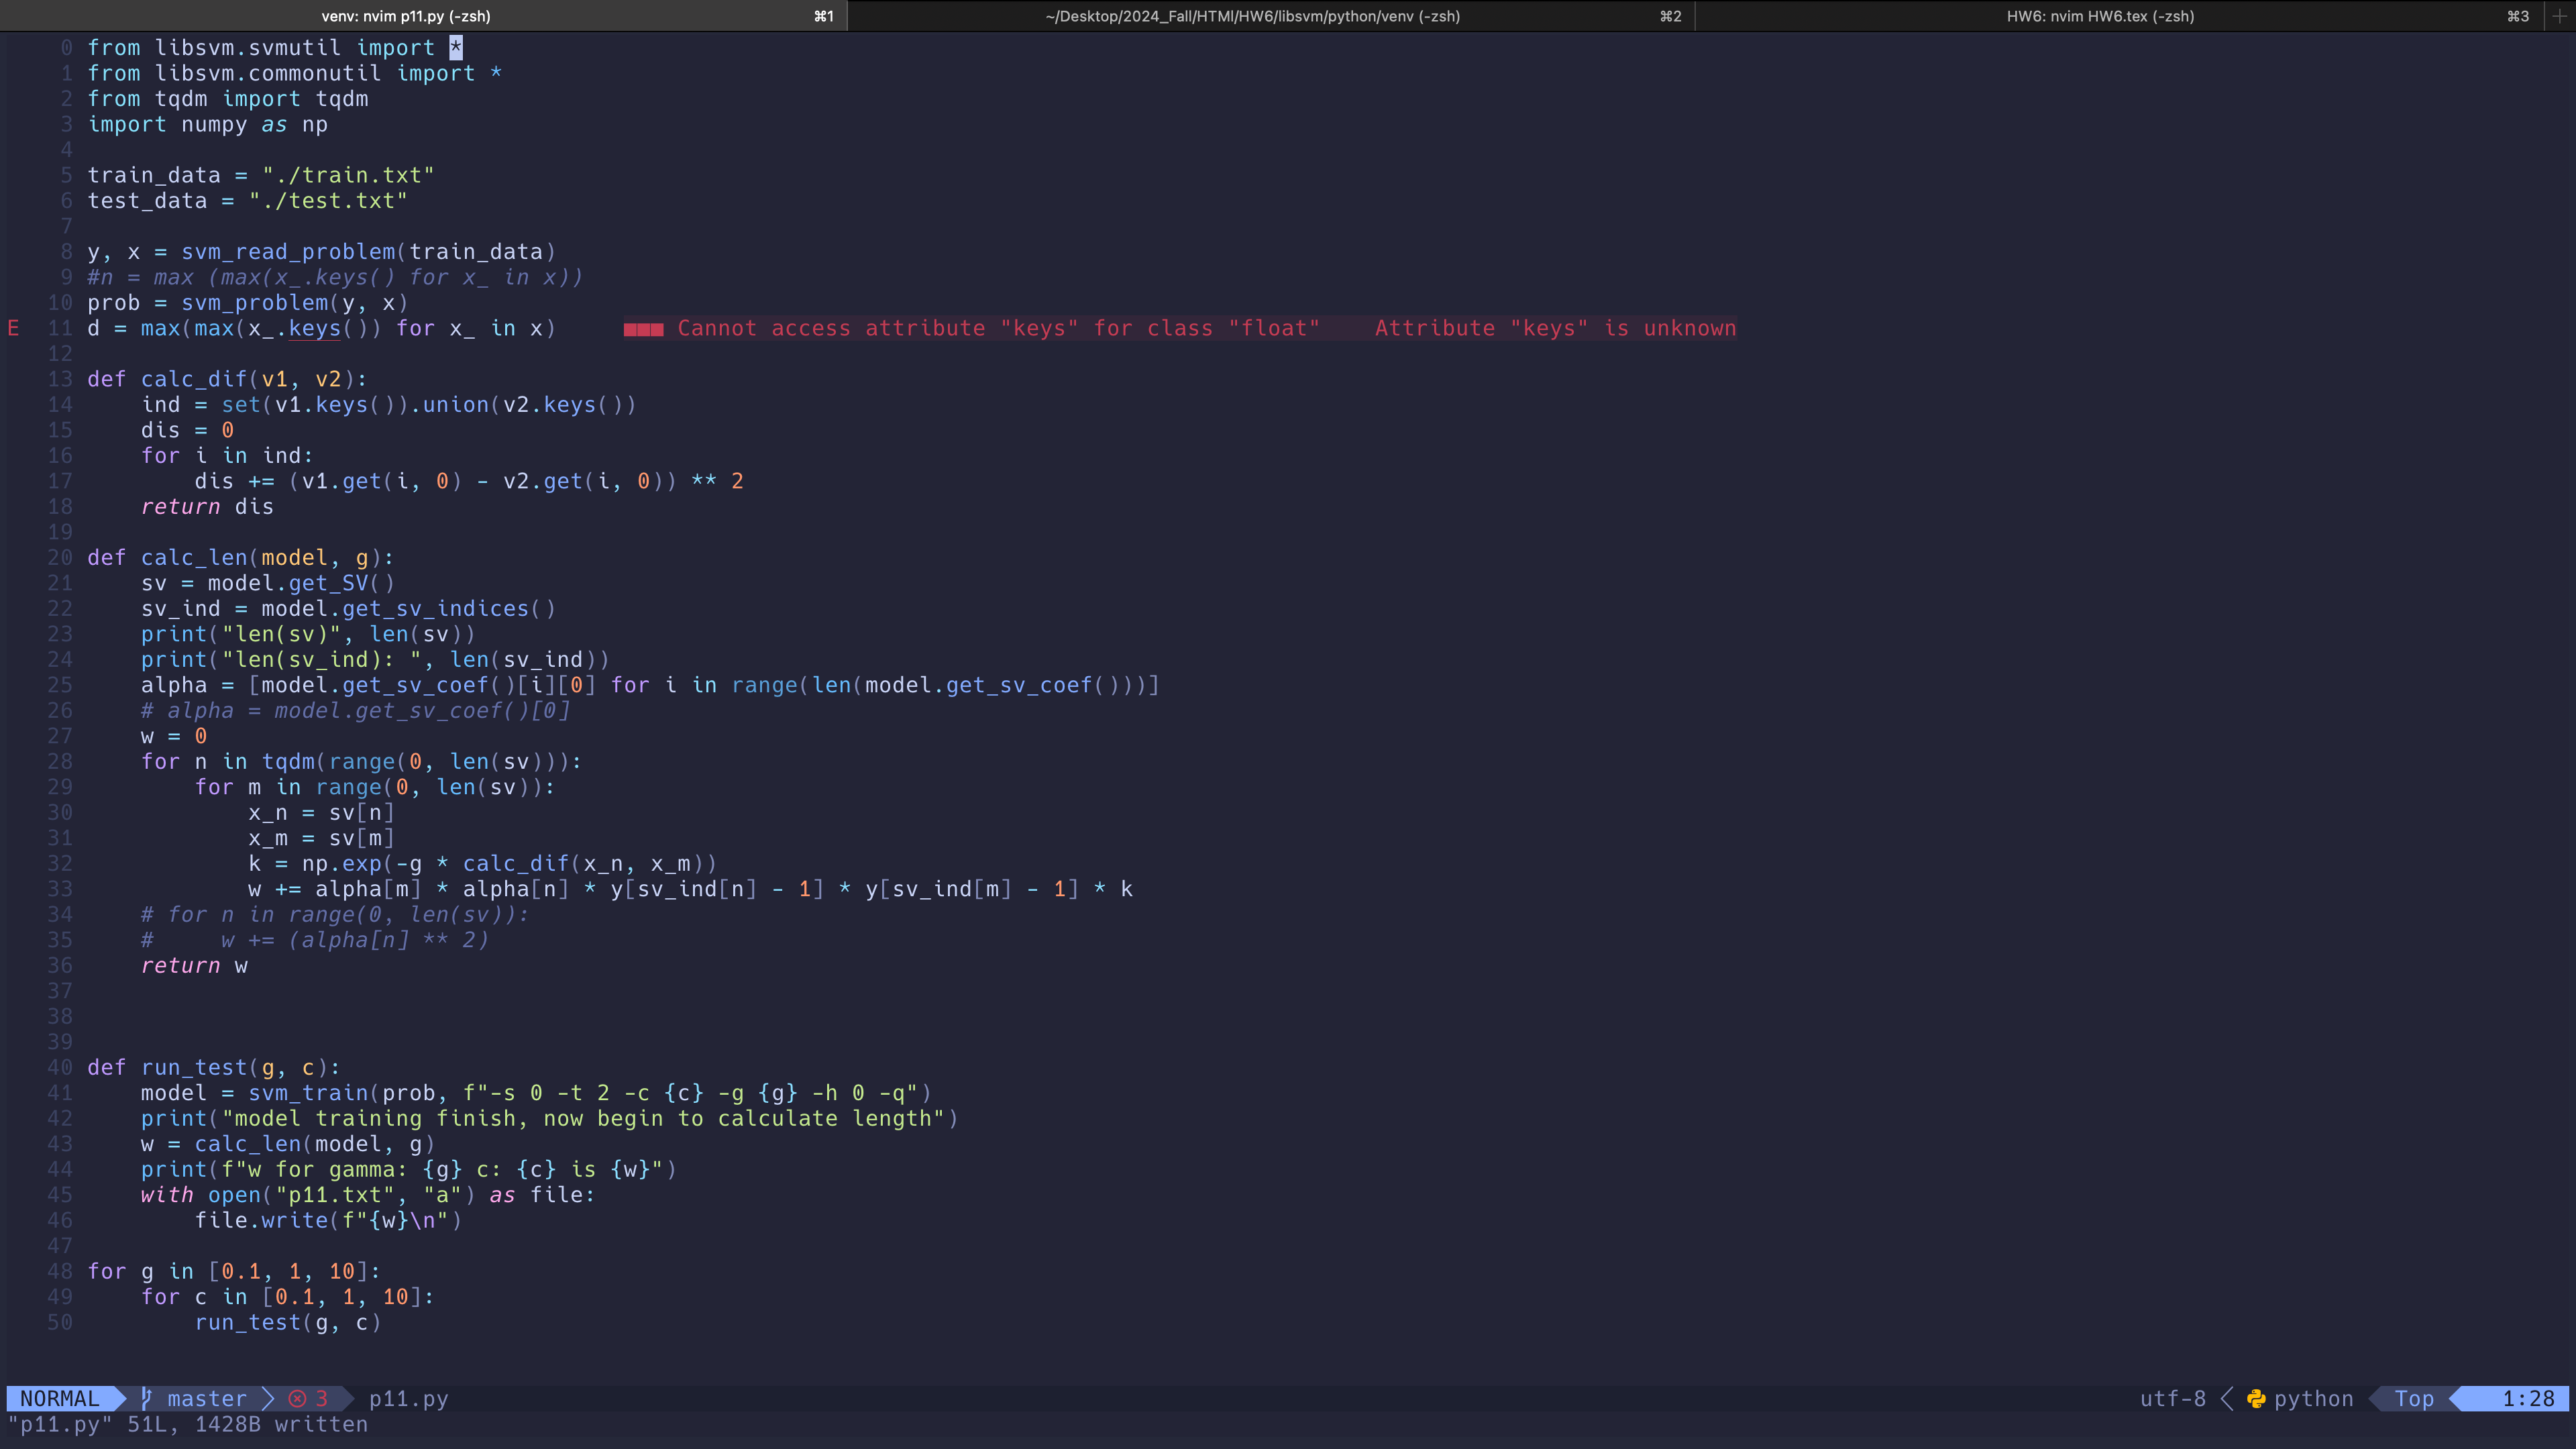
\includegraphics[width = \textwidth]{p11.png} \\
\newpage
\section*{11}
Table: \\
\begin{center}
\begin{tabular}{ |c|c|c|c| } 
 \hline
  \diagbox{$\gamma$}{C} & 0.1 & 1 & 10 \\
 \hline
  0.1 & 0.04127 & 0.01817 & 0.01779 \\ 
 \hline
  1 & 0.090780 & 0.0090780 & 0.0089836 \\
 \hline
  10 & 0.090793 & 0.0090793 & 0.0089819\\
 \hline
\end{tabular} \\ 
\end{center}
The number in each field of the table is the corresponding value of $\frac{1}{\norm{w}}$ \\ 
\par 
(Q, $\gamma$) = (0.1, 10) results in the largest margin. 0.090793 approximately \\ 
Findings: \\
\par
From the table we can see that the same $\gamma$, the margin is smaller with larger C. Also, for the same C, the margin is larger with larger $\gamma$. \\ 
These two phenomena can be explained separately. \\ 
First, larger C means that violation is penalized more. Also, we know that the soft-margin SVM finds a balance between maximizing the margin and minimizing violation. Therefore, a higher penalty for violation means that this balance leans more towards minimizing violation, and the priority for maximizing the margin becomes lower. So it is reasonable that compared with a model with small C, one with larger C results in a smaller margin. \\ 
Furthermore, we see that with fixed $\gamma$, $\frac{1}{\norm{w}}$ decreases quite significantly from $C = 0.1$ to $C = 1$, but from $C = 1$ to $C = 10$, $\frac{1}{\norm{w}}$ only decreases a little. This might be because that at $C = 1$ the penalty for violation is already sufficiently large, and there are only few cases of violation. Therefore, further increasing C to 10 does not result in a huge change in the training result, as there's not much room to further decrease the number of violations. \\ 
\par 
Second, larger $\gamma$ means that a more complex transform is used, and therefore the model has a higher degree of freedom when fitting the data vectors. Therefore, with a larger $\gamma$, the model can find a hyperplane that is further away from the data vectors, and hence the larger margin. \\
\newpage
Code Snapshot: \\
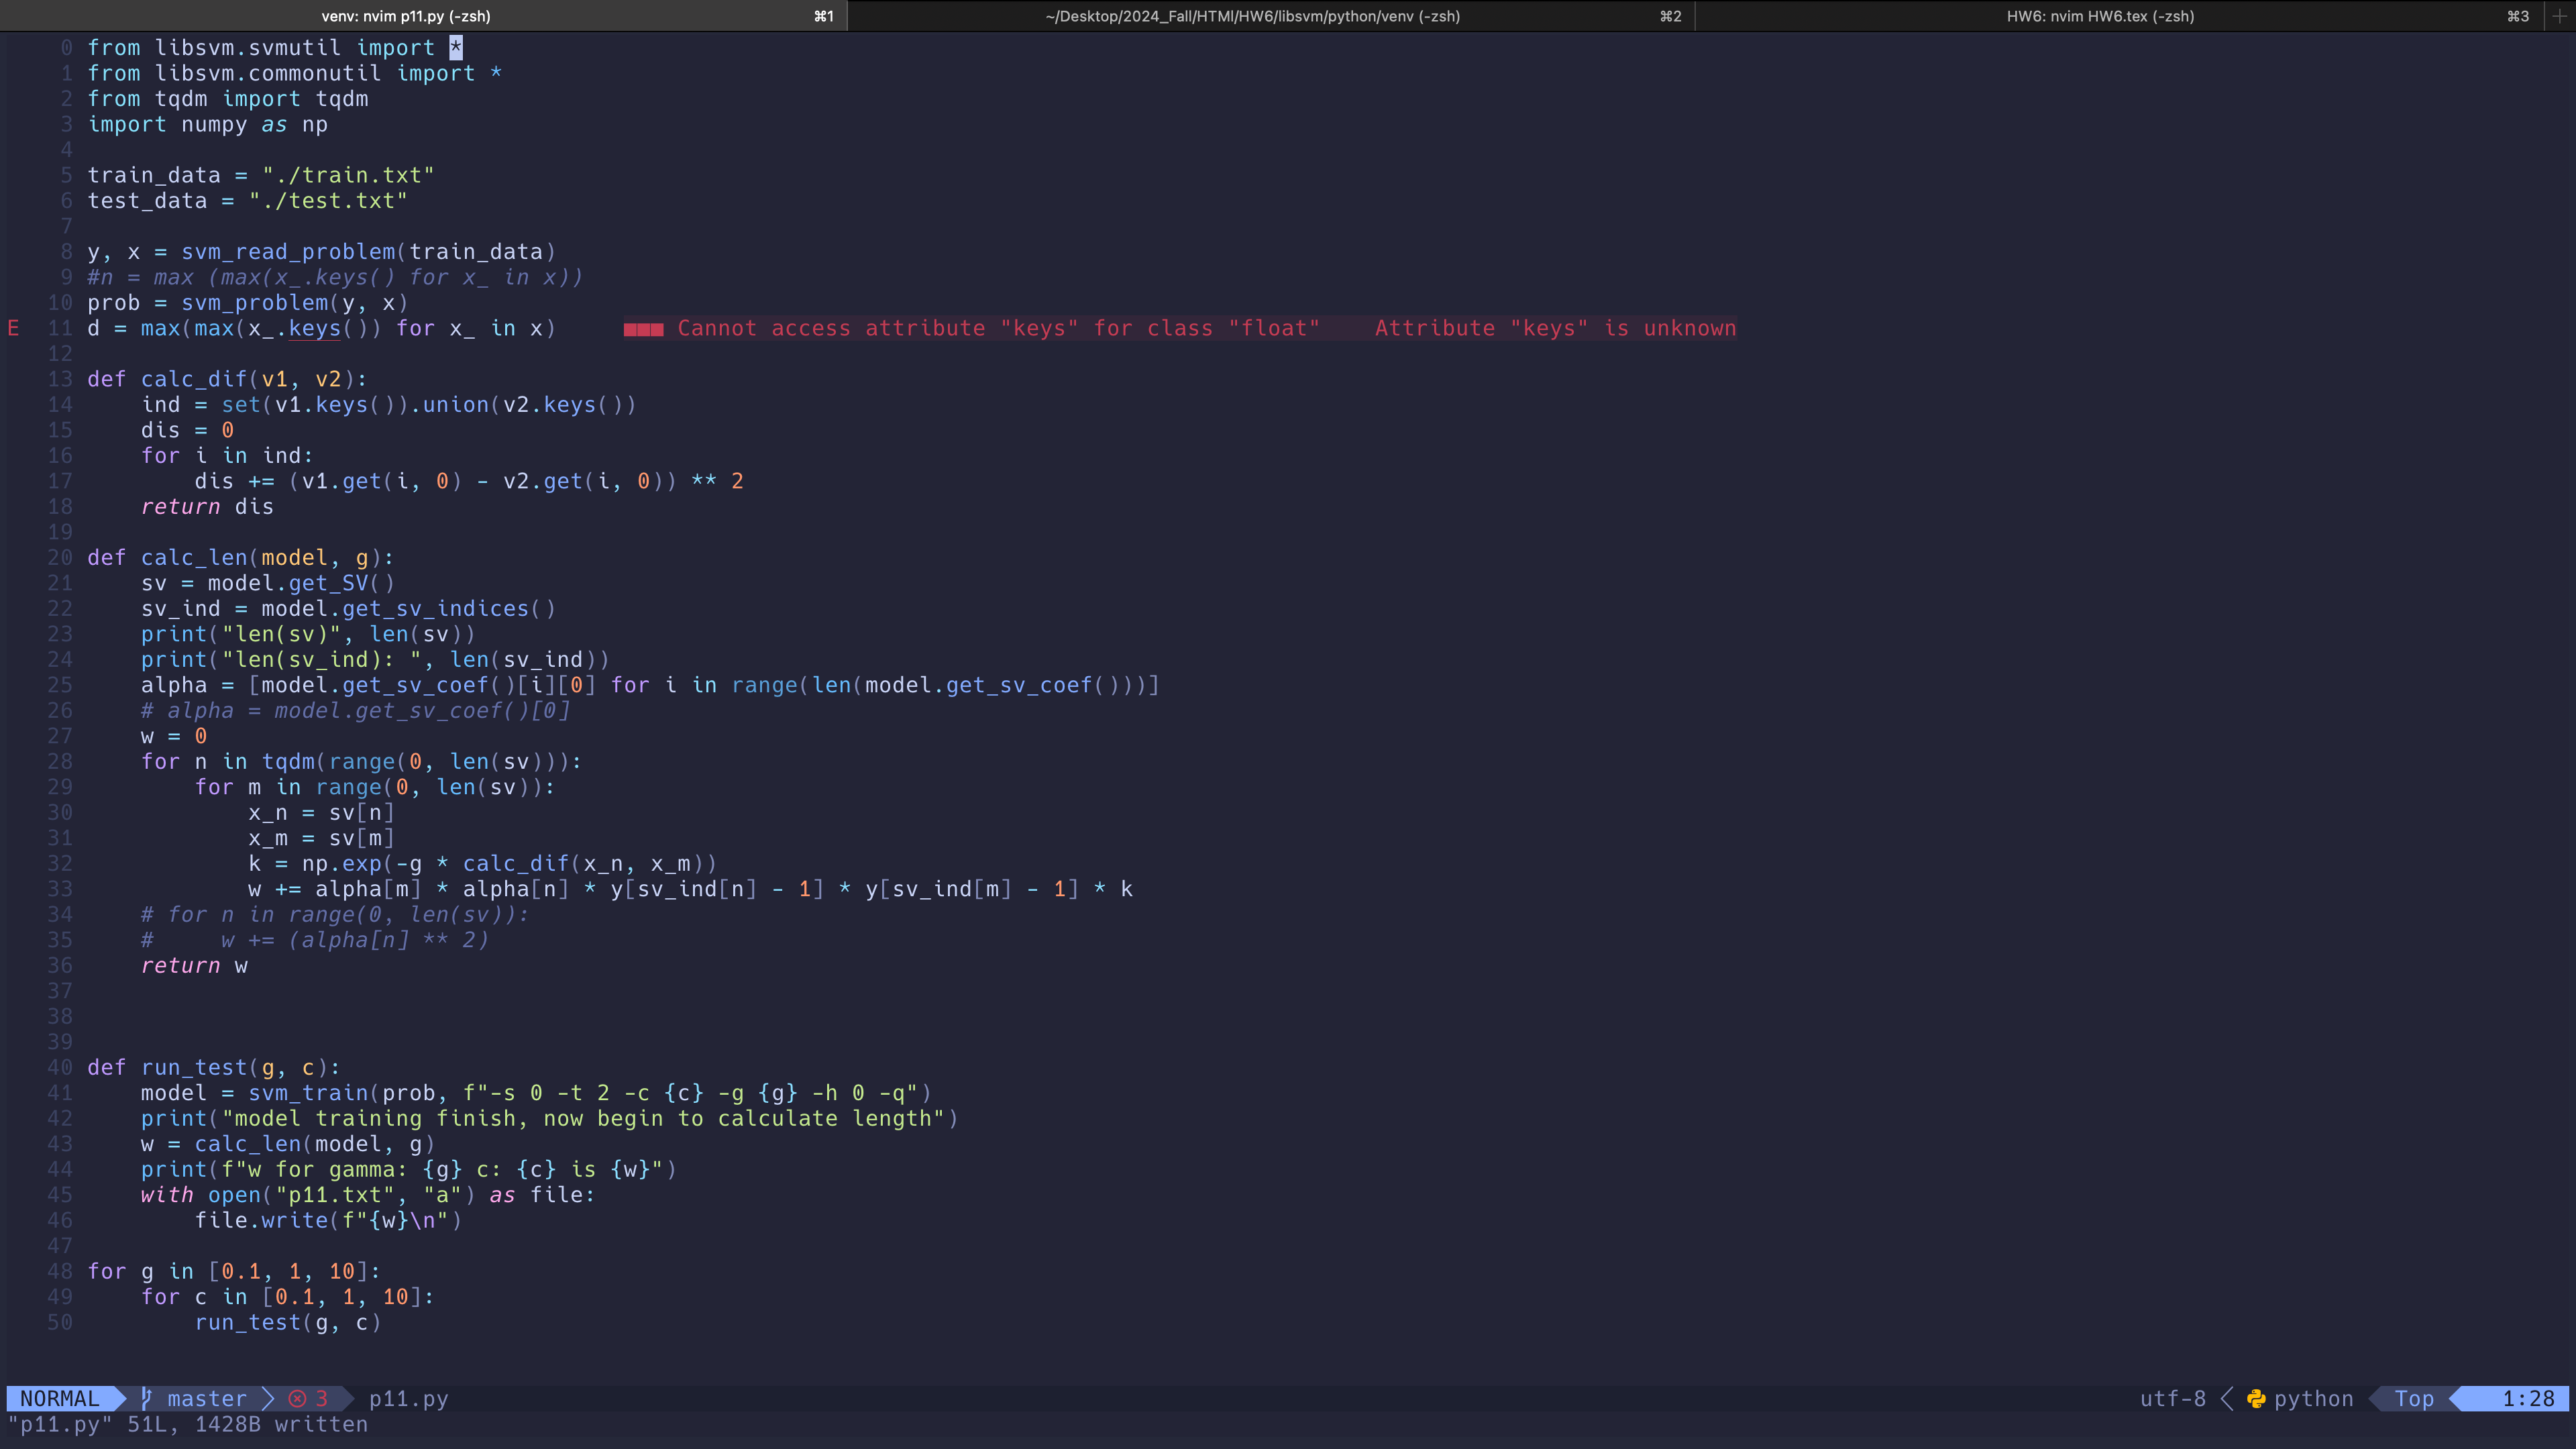
\includegraphics[width = \textwidth]{p11.png} \\
\newpage
\section*{12}
Histogram: \\ 
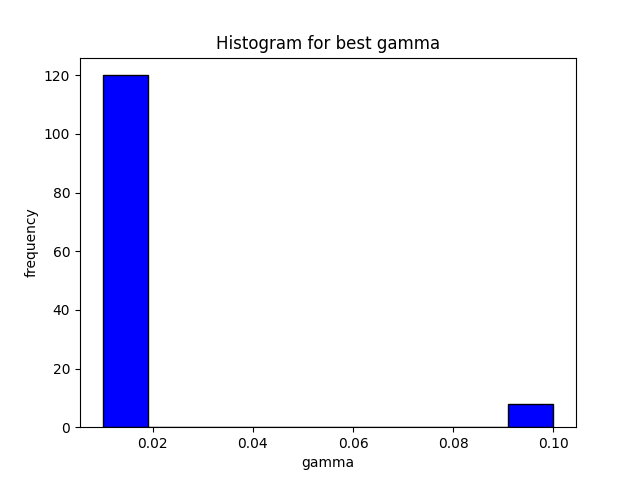
\includegraphics[width = \textwidth]{p12_fig.png} \\
\par 
Findings: \\ 
\par
From the histogram above we see that value of the best $\gamma$ is either 0.01 or 0.1. Moreover, the overwhelming majority is 0.01, with 120 out of 128 values of best $\gamma$ being 0.01. \\ 
A possible explanation to this phenomenon is that when adopting validation, an overfitting model is punished in the model selection step. That is a model that overfits is likely to have high $E_\text{val}$ and wouldn't be chosen. As we're taught in class, a larger $\gamma$ in the Gaussian kernel means that there are more effective terms in the transform, and a more complex model is therefore allowed. Therefore, overfitting is more likely to occur, and the model's classifying performance judging by $E_\text{eval}$ is likely to be worse. As a result, out of the 128 experiments, most of the time the model with the lowest $\gamma$ factor in the Gaussian kernel performs the best, as it's less prone to overfitting. \\ 
Nevertheless, the few cases where $\gamma = 0.1$ performs better then $\gamma = 0.01$ still implies that sometimes a more complex model does have better classifying performance. \\
Code Snapshot: \\ 
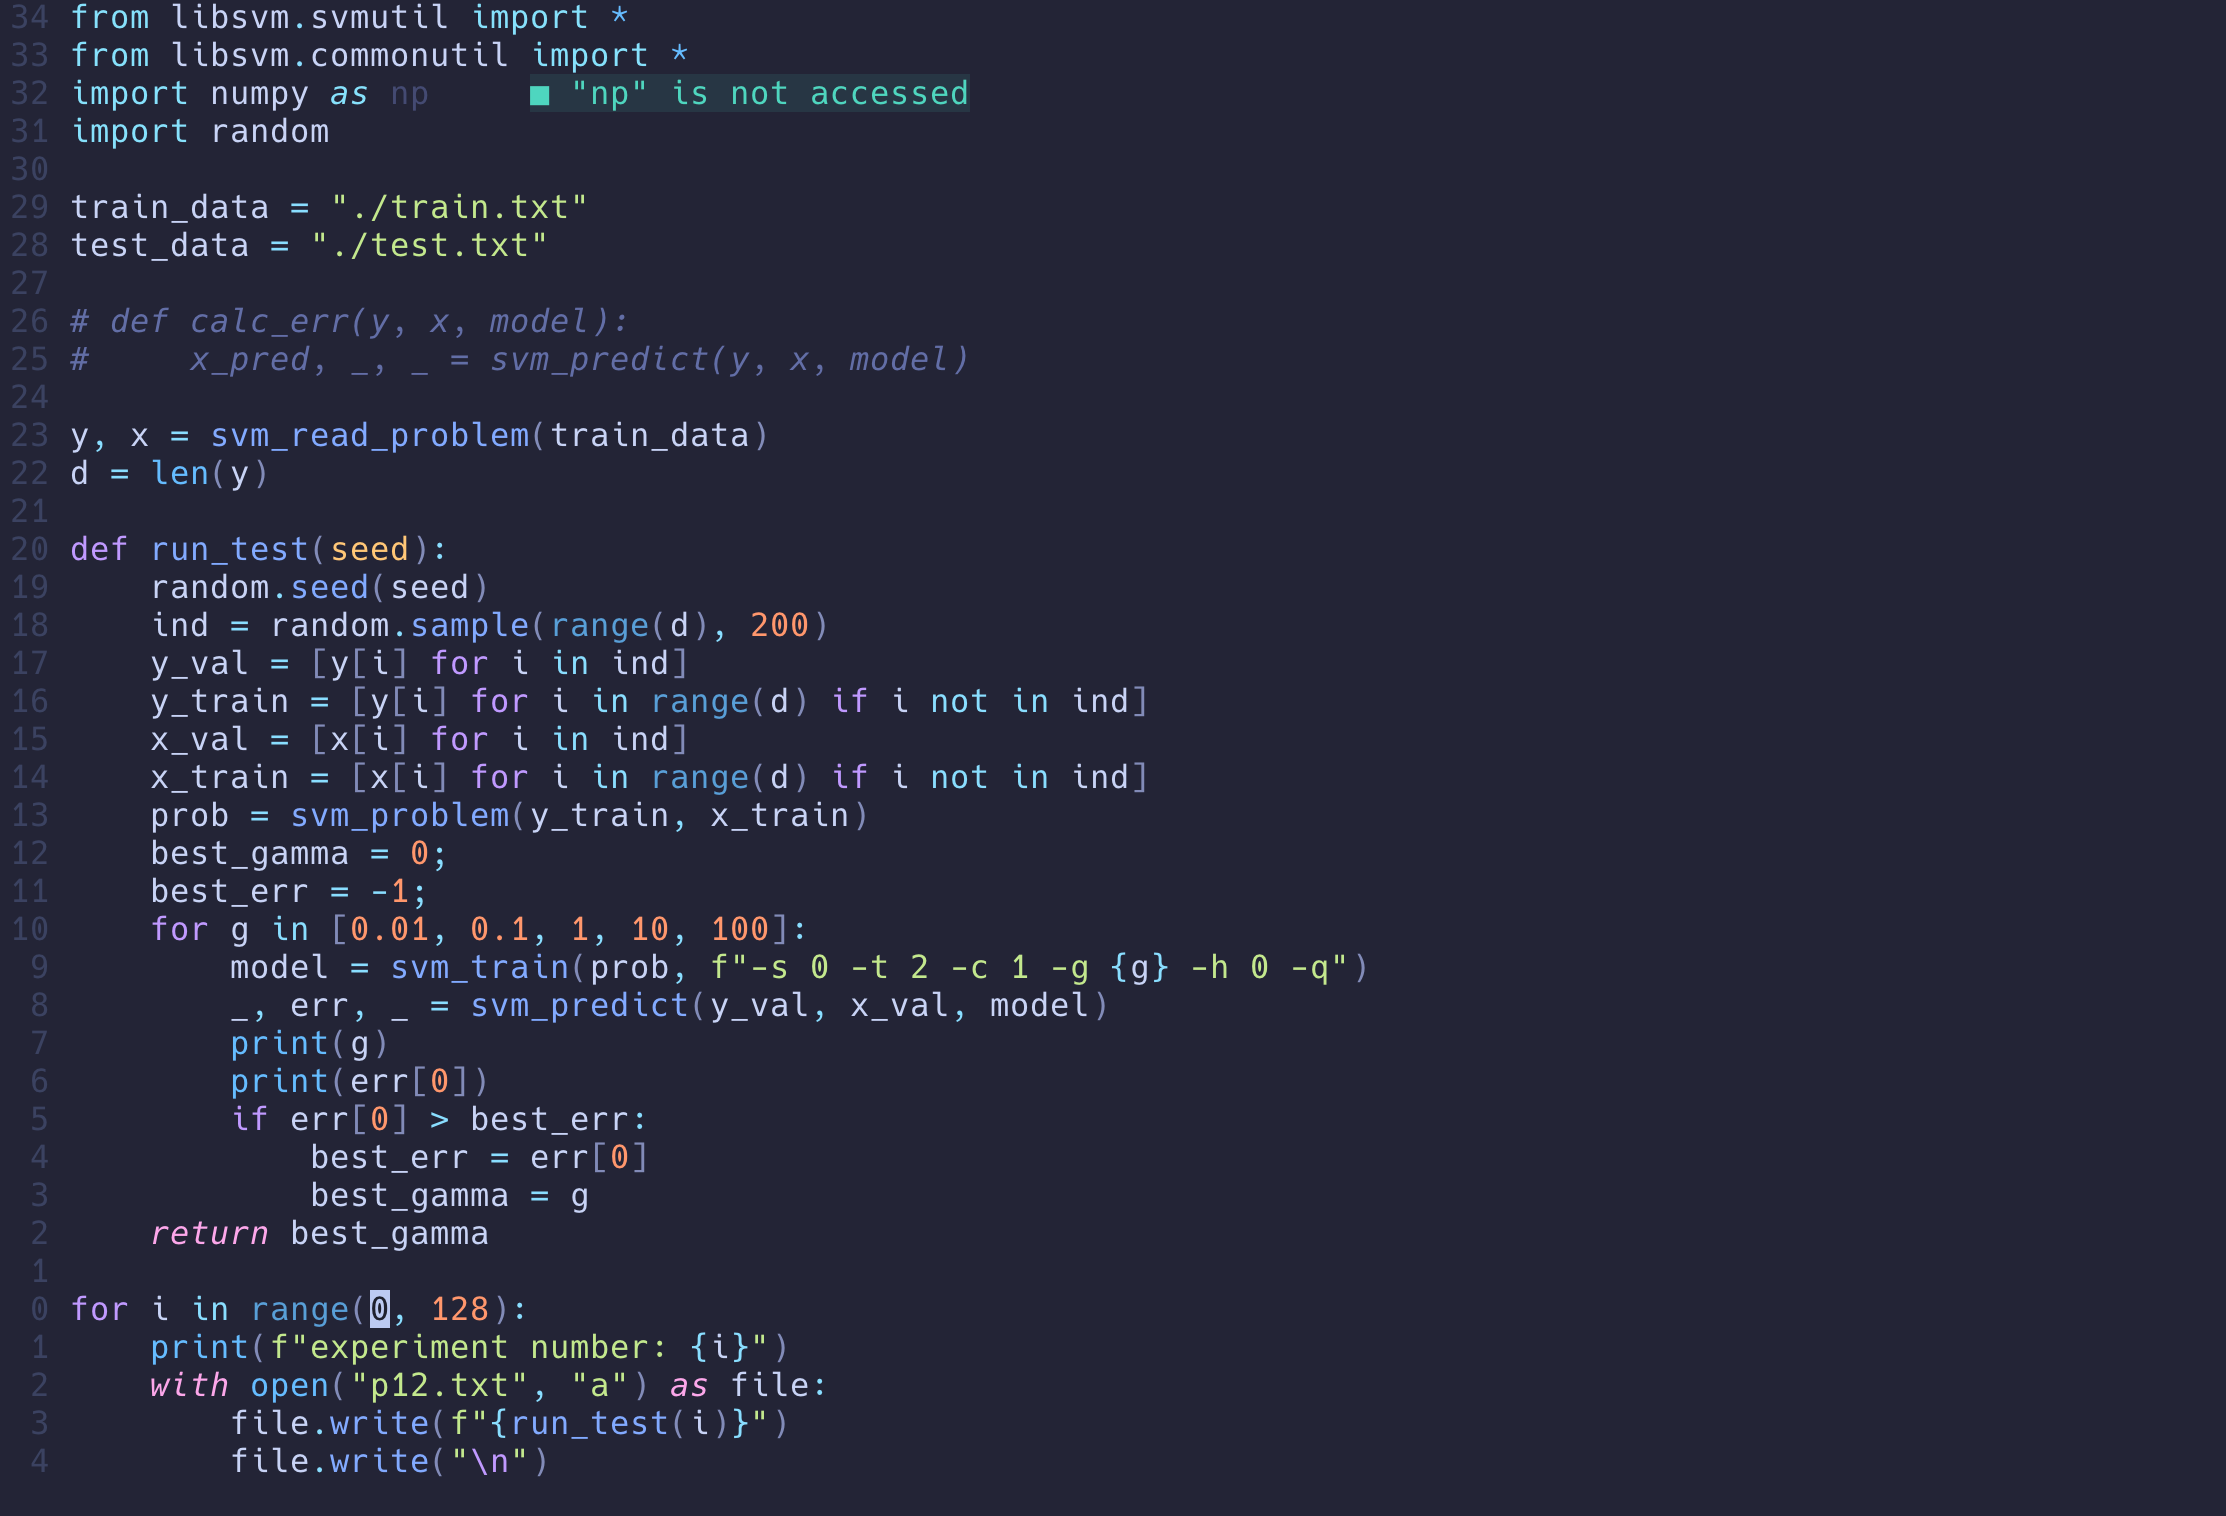
\includegraphics[width = \textwidth]{p12.png}
\end{document}
